\documentclass[UTF8,AutoFakeBold,twoside,fontset=fandol]{CarlosTexArt}

% ============  配置区  ============ %
\title{科技论文模板}
\author{Carlos QU\\ccandle@foxmail.com}

% 如需子图排版，取消下行注释
% \usepackage{subcaption}

\begin{document}

%% 编译说明：
%%  默认 recipe "xelatex"：适合只改内容不改参考文献的情况
%%  修改了参考文献后，请切换 recipe "xebibitex" 全量编译
%%  VS Code 中：Ctrl+Alt+B 编译，Ctrl+Alt+V 预览 PDF
\bibliographystyle{gbt7714-numerical}
\maketitle

\begin{abstract}[keyword1][keyword2]
    本文是一个科技论文写作模板，基于 XeLaTeX 编译，适用于 Windows、macOS 和 Linux 下的 VS Code +
    LaTeX Workshop + TeX Live/MacTeX 环境。

    在 \texttt{abstract} 环境的方括号参数中按顺序填写关键词，
    最多支持 5 个关键词，如 \texttt{\textbackslash begin\{abstract\}[关键词1][关键词2][关键词3]}。
\end{abstract}


% ============  正文从此开始  ============ %
% 每一章在 ./page 下新建 .tex 文件，用 \include 或 \input 引入
% \include 会自动分页，\input 则连续排版
\section{引言}

这是论文正文。章节标题使用 \verb|\section{}| 命令，会自动编号。

\subsection{子章节}

子章节用 \verb|\subsection{}| 命令。
引用公式用 \verb|\autoref{eq:example}|，例如 \autoref{eq:example}。

\begin{equation}
    E = mc^2
    \label{eq:example}
\end{equation}

\subsection{图表示例}

如图 \autoref{fig:sample} 所示，插图直接放在 \texttt{img/} 目录下。

\begin{figure}[H]
    \centering
    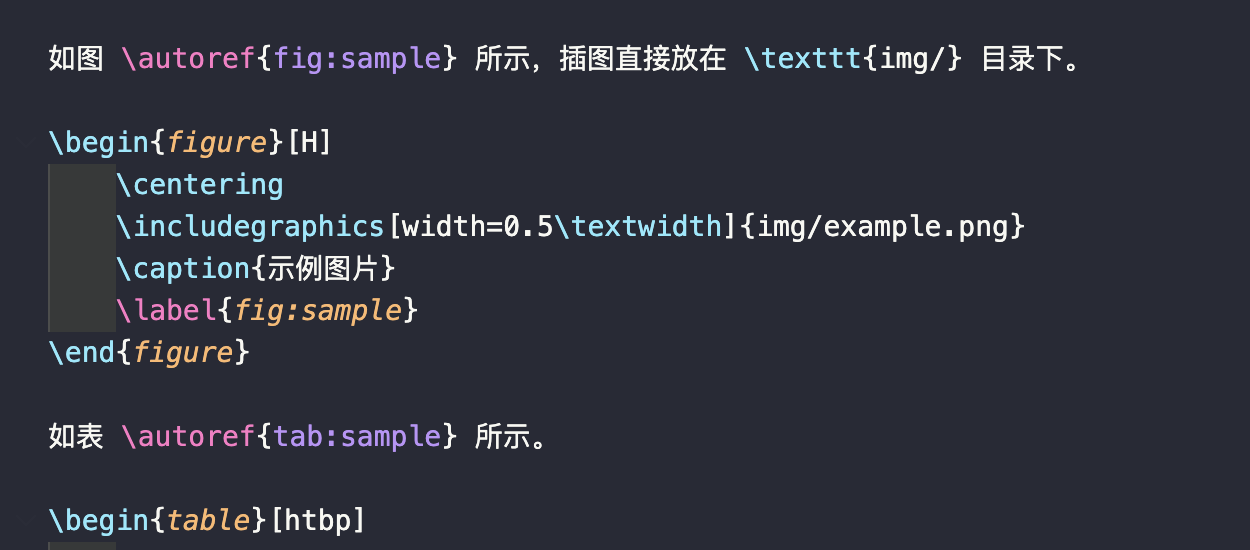
\includegraphics[width=0.5\textwidth]{img/example.png}
    \caption{示例图片}
    \label{fig:sample}
\end{figure}

如表 \autoref{tab:sample} 所示。

\begin{table}[htbp]
    \centering
    \caption{示例表格}
    \begin{tabular}{ccc}
        \hline
        参数 & 符号 & 数值 \\
        \hline
        电阻 & $R$ & $10\Omega$ \\
        电容 & $C$ & $100\mu$F \\
        \hline
    \end{tabular}
    \label{tab:sample}
\end{table}

\subsection{参考文献引用}

使用 \verb|\cite{}| 引用文献，如 \cite{latex-intro} 和 \cite{vscode-latex}。

\section{结论}

本文提供了一个简洁的科技论文写作模板。


\newpage
\bibliography{doc/bibfile}

\newpage
\begin{appendix}
    \section{补充材料}
    附录内容写在这里。
\end{appendix}

\end{document}
